\documentclass[10pt, conference, compsocconf]{IEEEtran}

\fontfamily{cmr}\selectfont
\renewcommand{\sfdefault}{cmss}
\renewcommand{\rmdefault}{cmr}
\renewcommand{\ttdefault}{cmtt}
\usepackage[utf8]{inputenc}
\usepackage[russian]{babel}


\usepackage{minted}
\usepackage{verbments}

\usepackage{algpseudocode}
\usepackage{algorithm}
\usepackage{algorithmicx}
\usepackage{graphicx}
\usepackage{caption}

\renewcommand\IEEEkeywordsname{Ключевые слова}
\renewcommand\listingscaption{Листинг}

\hyphenation{op-tical net-works semi-conduc-tor}

\begin{document}

\algtext*{EndWhile}% Remove "end while" text
\algtext*{EndIf}% Remove "end if" text
\algtext*{EndFor}% Remove "end for" text
\algtext*{EndFunction}% Remove "end function" text

\title{Лексический анализ динамически формируемых строковых выражений}

\author{\IEEEauthorblockN{Полубелова Марина Игоревна}
\IEEEauthorblockA{Санкт-Петербургский Государственный Университет\\
Санкт-Петербург, Россия\\
polubelovam@gmail.com}
\and
\IEEEauthorblockN{Григорьев Семён Вячеславович}
\IEEEauthorblockA{Санкт-Петербургский Государственный Университет\\
Санкт-Петербург, Россия\\
Semen.Grigorev@jetbrains.com}
}

\maketitle


\begin{abstract}
Строковые выражения могут использоваться для формирования и последующего исполнения кода во время выполнения основной программы. Такой подход обладает высокой выразительностью, однако затрудняет разработку, отладку и сопровождение, а также является источником таких уязвимостей как внедрение SQL и межсайтовый скриптинг. Статический анализ строковых выражений предназначен для борьбы с недостатками подхода посредством проверки, что все формируемые выражения удовлетворяют некоторым свойствам, без запуска программы. Лексический анализ или токенизация формируемого кода является важным шагом такого статического анализа. В данной статье будет описан автоматизированный подход к созданию лексических анализаторов динамически формируемого кода, который позволит упростить создание инструментов, предназначенных для статического анализа такого кода.
\end{abstract}

\vspace{5 mm}
\begin{IEEEkeywords}
 анализ строковых выражений, генератор лексических анализаторов, лексический анализ, встроенные языки, string analysis, lexing, string-embedded language
\end{IEEEkeywords}

\IEEEpeerreviewmaketitle

\section{Введение}

Многие языки программирования позволяют работать со строковыми выражениями. Они могут формироваться динамически с использованием строковых операций и языковых конструкций, например, условных операторов и циклов. Такие выражения широко используются в программных интерфейсах ODBC, ADO.NET, JDBC, предназначенных для формирования запросов к базе данных в языках программирования C++, C\#, Java, соответственно, а также в web-программировании. Некоторые примеры использования динамически формируемых строковых выражений представлены в листингах~\ref{lst:verbments1}, \ref{lst:verbments2}. 

\begin{listing}[h]
\begin{pyglist}[language=csharp,numbers=none,numbersep=5pt]
 private void Go(bool cond)
 {
   string tableName = cond ? "Sold " : "OnSale ";
   string query =
       "SELECT ProductID, UnitPrice, ProductName" 
           + " FROM dbo.products_" + tableName
           + " WHERE UnitPrice > 1000 "
           + " ORDER BY UnitPrice DESC;";
   Program.ExecuteImmediate(query);
 }
\end{pyglist}
\caption{Пример встроенного SQL в C\#}
\label{lst:verbments1}
\end{listing}


\begin{listing}[h]
\begin{pyglist}[language=php,numbers=none,numbersep=5pt]
<?php
//Embedded SQL
$query = 'SELECT * FROM '. $my_table;
$res = mysql_query($query);
//HTML markup generation
echo "<table>\n";
while($line=mysql_fetch_array($res, MYSQL_ASSOC)){
echo "\t<tr>\n";	
foreach ($line as $col_value){
echo "\t\t<td>$col_value$</td>\n";}
echo "\t</tr>\n";}
echo "</table>\n";
?>
\end{pyglist}
\caption{Использование нескольких встроенных в PHP языков (MySQL, HTML)}
\label{lst:verbments2}
\end{listing}


Динамически формируемые строковые выражения воспринимаются компилятором как обычные строки, что усложняет разработку и сопровождение системы. Во-первых, о наличии ошибок таких, как лексических или синтаксических, в сформированном выражении становится известно только в момент выполнения программы, когда оно начинает выполняться в своем программном окружении. Во-вторых,  при ненадлежащей обработке пользовательского ввода система становится уязвимой, например, для SQL инъекций или межсайтового скриптинга. Указанные проблемы можно решить, включив обработку строковых выражений в статический анализ программы. 

Классическим подходом к статическому анализу является проведение лексического анализа и синтаксического разбора исходного кода. Синтаксический анализ строит структурное представление, которое используется в дальнейшем, например, для семантического анализа или трансформаций, проводимых в контексте реинжиниринга. В рамках данного подхода широко распространен автоматизированный способ создания лексических и синтаксических анализаторов такими генераторами как Lex, Yacc и их потомками. Использование подобных инструментов сокращает затраты на создание программных продуктов, требующих построения структурного представления кода. Однако существующие генераторы лексических и синтаксических анализаторов не применимы для создания инструментов обработки динамически формируемого кода из-за того, что такой код, как правило, не представим в виде линейного потока, принимаемого на вход классическими анализаторами. 
% * <Екатерина Вербицкая> 20:04:18 13 Aug 2015 UTC+0300:
% > Классическим подходом к статическому анализу является проведение лексического анализа и синтаксического разбора исходного кода.
% 
% Лексический и синтаксический анализ это не подходы к статическому анализу, а то, что делается до того, как статический анализ начинает осуществляться.
% ^ <Марина Полубелова> 10:42:59 14 Aug 2015 UTC+0300:
% Не всегда ведь. Например, анализ потока данных -- это ведь тоже статический анализ, но для него не надо проводить лексический и синтаксический анализ. Можно переформулировать предложение: "В статический анализ исходного кода обычно входит лексический и синтаксический анализ."
% ^ <Екатерина Вербицкая> 23:12:51 14 Aug 2015 UTC+0400:
% Обычно такие анализы проводятся над деревом синтаксического разбора. Иначе сложно, ведь ты не знаешь, что эти буквы в текстовом файле означают.
% ^ <Марина Полубелова> 10:36:31 15 Aug 2015 UTC+0300:
% "Лексический и синтаксический анализ являются необходимым шагом для проведения статического анализа исходного кода."

Таким образом, есть необходимость в создании генератора лексических анализаторов для динамически формируемого кода, который предоставляет функциональность, аналогичную классическому. Это позволит упростить создание инструментов, которые предназначены для решения задач, возникающих при обработке динамически формируемого кода. Примерами таких задач являются трансформация запросов с одного языка на другой, возникающая в контексте реинжиниринга информационных систем, подсветка синтаксиса и ошибок в интегрированных средах разработки, а также подсчет различных метрик.  
 
В данной статье будет описан автоматизированный подход создания лексического анализатора для динамически формируемого кода. В рамках работы были разработаны алгоритм лексического анализа и генератор лексических анализаторов,  за основу которого была взята библиотека FsLex~\cite{FsLex}. Указанные компоненты были реализованы как часть проекта  YaccConstructor~\cite{YC_article}, который является модульным инструментом для проведения лексического анализа и синтаксического разбора, а также платформой для поддержки встроенных языков.


\section{Обзор}

В данном обзоре рассматриваются существующие инструменты, предназначенные для работы с динамически формируемыми выражениями, генератор лексических анализаторов FsLex и проект YaccConstrucor, в котором ведется разработка автоматизированного подхода создания лексических анализаторов для динамически формируемого кода. 


\subsection{Обзор существующих инструментов}

Для работы с динамически формируемыми строковыми выражениями существует ряд инструментов. Почти все они предназначены для решения какой-то одной конкретной задачи: либо проверка выражения на соответствие описанию некоторой эталонной грамматики,  либо статический анализ программы на уязвимость. Так как генерация всех значений динамически формируемого выражения значительно снижает скорость проведения анализа и возможны ситуации, когда количество принимаемых выражением значений может быть бесконечным, то  целесообразно иметь конечное представление множества значений данного выражения и уже над ним проводить анализ. 

Конечное представление множества значений строкового выражения впервые было использовано в инструменте Java String Analyzer~\cite{JSA}. Этот инструмент предназначен для анализа строк и строковых операций в Java-программе. Результатом этого приближения стал конечный автомат, который используется для проверки включения языков: проверяется включение языка, порождаемого программой, в язык, описанный пользователем. Затем инструмент PHP String Analyzer~\cite{PHPSA}, использовав идею предыдущего инструмента, уточнил проводимую аппроксимацию, результатом которой стала контекстно-свободная грамматика. Этот инструмент применяется для статической валидации HTML-страниц, генерируемых в PHP-программе. 

В инструменте Pixy~\cite{Pixy}, предназначенном для поиска SQL инъекций  и межсайтового скриптинга в PHP-программах, применяется техника path pruning, позволяющая проводить анализ только тех значений строкового выражения, которые оно может принять в момент выполнения программы Инструмент Stranger~\cite{Stranger} расширяет указанный подход, используя в качестве структурного представления динамически формируемого кода конечный автомат над алфавитом символов обрабатываемого языка. При этом рассматривается общий случай: когда аргументами строковых операций являются конечные автоматы. В рамках инструмента Stranger разработан алгоритм, который вычисляет результат этих операций и возвращает его в виде конечного автомата, что позволяет достичь более высокой точности анализа по сравнению с аналогами.  

Разработчики следующего инструмента расширили круг решаемых задач, сформулировав вопросы  безопасности, корректности и производительности сформированных запросов с использованием таких программных интерфейсов, как ADO.NET и JDBC. Описание этого инструмента дается в статье~\cite{StaticFrame}, в которой также была указана разработанная функциональность: поиск SQL инъекций, извлечение множества всех значений для строкового выражения, удаление неиспользуемых переменных в формируемом запросе, а также проверка на соответствие типов возвращаемого запросом значения с ожидаемым в программе.  

Инструмент SAFELI~\cite{SAFELI}, также предназначенный для поиска уязвимостей в web-приложениях, отличается от рассмотренных тем, что структурным представлением динамически формируемого кода является синтаксическое дерево разбора. Результат получается посредством сопоставления полученного дерева с синтаксическим деревом шаблона уязвимости, параметризованного реальными данными. Однако SAFELI не поддерживает обработку строковых выражений, которые могут быть получены при участии строковых операций. 

Для проведения лексического анализа и синтаксического разбора множества значений строкового выражения был разработан инструмент Alvor~\cite{Alvor}, который является расширением для среды разработки Eclipse, предназначенным для статической валидации SQL-выражений, встроенных в программы на Java. Одной из  возможностей инструмента является поиск лексических и синтаксических ошибок, однако поддержка нового языка генерируемого кода является нетривиальной задачей из-за отсутствия генераторов лексических и синтаксических анализаторов. Кроме того, Alvor не поддерживает обработку выражений, полученных с помощью строковых операций (кроме конкатенации) и циклов. 

\subsection{Инструмент YaccConstructor}

YaccConstructor~\cite{YC_article} является модульным инструментом с открытым исходном кодом~\cite{YCrepo}, предназначенным для исследований в области лексического анализа и синтаксического разбора, а  также платформой для поддержки встроенных языков~\cite{YC_SECR}. Данный инструмент реализован на платформе Microsoft .NET, основной язык разработки --- F\#.  

Разработанный механизм анализа встроенных языков ранее имел ограничения на структуру динамически формируемого выражения: лексический и синтаксический анализаторы могли обрабатывать только аппроксимацию, представленную в виде ориентированного ациклического графа (DAG). Это не позволяло корректно обрабатывать выражения, полученные с помощью циклов.
	
В данной работе такое ограничение снимается: лексический анализатор работает с произвольным конечным автоматом над алфавитом символов обрабатываемого языка. Разработанный модуль для лексического анализа, который состоит из генератора лексических анализаторов и интерпретатора, соответствующего предложенному алгоритму лексического анализа, внедрен в инструмент YaccConstructor.    

\subsection{Генератор лексических анализаторов FsLex}

При проведении лексического анализа часто используются генераторы лексических анализаторов, которые по спецификации обрабатываемого языка строят описание конечного преобразователя, на основе которого входной поток символов преобразуется в поток токенов. Для реализации инструмента для проведения лексического анализа динамически формируемого кода был выбран генератор лексических анализаторов FsLex~\cite{FsLex}. Этот выбор обусловлен тем, что реализованный механизм является компонентом инструмента YaccConstructor, основным языком разработки которого является язык программирования F\#. 

Генератор лексических анализаторов на вход принимает файл с расширением .fsl, в котором описана лексическая спецификация  языка, формат определения которой представлен в листинге~\ref{lst:format} .


\fvset{frame=lines,framesep=5pt}
\begin{listing}[H]
\begin{pyglist}[language=csharp,numbers=none,numbersep=5pt]
{
module Lexer
// header: any valid F# code can appear here
open Parser //specifies type of tokens 
}
// regex macros 
let ident = regexp ... 
// rules   
rule entrypoint = parse
| regexp { action }
| ... 
and entrypoint = parse
...
\end{pyglist}
\caption{Формат определения спецификации для языка}
\label{lst:format}
\end{listing}


В описании спецификации выделяется три блока: заголовок (\verb|header|), блок именованных регулярных выражений и блок точек вхождения (\verb|entrypoint|). 

Обычно заголовок содержит директивы \verb|open|, необходимые для выполнения действий (\verb|action|), а также вспомогательные функции. Между заголовком и точками вхождений можно определять имена для регулярных выражений. Для каждой точки вхождения генерируется функция на языке F\# с таким же именем. Аргументом для таких функций является буфер лексических анализаторов, а возвращают они вычисленное действие. При этом возвращаемое значение должно иметь тип \verb|Parser.token|, который описывает токены. 

Буфер лексических анализаторов --- это абстрактный тип данных,  реализованный в модуле стандартной библиотеки \verb|Lexing| (Microsoft.FSharp.Text.Lexing). Mетоды \verb|FromString|, \verb|FromBytes|, \verb|FromChars| создают лексические буферы, принимающие данные из строки символов, массива  байтов и символов, соответственно. Данный тип позволяет сохранять для лексемы координаты отступов начала и конца в исходном коде и накопленную строку. 

Лексический анализатор читает символы из буфера и сравнивает их с регулярным выражением, которое соответствует правилу, до тех пор, пока префикс не совпадает с одним  из регулярных выражений. Если префикс совпадает с несколькими регулярными выражениями, то из них выбирается то, которое первым определено в спецификации. Например, если у нас есть два правила, которые на выражения ``*'' и ``**'' должны возвращать токены \verb|MULT| и \verb|POW|, соответственно, то в определении спецификации необходимо сперва указать правило для токена \verb|POW|, а только потом для токена \verb|MULT|. После выбора регулярного выражения, к накопленной строке применяется действие, соответствующее этому регулярному выражению. 

Пример спецификации для языка арифметических выражений представлен в листинге~\ref{lst:calcSpec}.

\fvset{frame=lines,framesep=5pt}
\begin{listing}[h]
\begin{pyglist}[language=csharp,numbers=none,numbersep=5pt]
{
module Calc.Lexer
open Calc.Parse 
open Microsoft.FSharp.Text.Lexing

let lexeme lb = LexBuffer<_>.LexemeString lb
}

let digit = ['0'-'9']
let whitespace = [' ' '\t' '\r' '\n']

rule token = parse
| whitespace { token lb }
| ['-']? digit+ ('.'digit+)? (['e' 'E'] digit+)?
       { NUMBER(lexeme lb) }
| '-'  { MINUS(lexeme lb) }
| '/'  { DIV(lexeme lb) }
| '+'  { PLUS(lexeme lb) }
| "**" { POW(lexeme lb) }
| '*'  { MULT(lexeme lb) }

\end{pyglist}
\caption{Лексическая спецификация для языка арифметических выражений}
\label{lst:calcSpec}
\end{listing}

Результатом работы генератора является файл с расширением .fs с кодом F\# для лексического анализатора. Этот файл содержит код, указанный в заголовке спецификации, конечный преобразователь и функции, которые были созданы на каждую точку вхождения, а также вызов функции интерпретатора построенного конечного преобразователя. Для того чтобы использовать такой лексический анализатор, полученный файл вместе с описанием типов токенов, которые автоматически строятся по грамматике эталонного языка, необходимо добавить в модуль, предназначенный для лексического анализа. 

%\subsection {Выводы}

\section{Лексический анализ}
Основной задачей лексического анализа является преобразование входного потока символов в поток токенов, соответствующих спецификации обрабатываемого языка, и сохранение привязки лексических единиц к исходному коду. В классическом лексическом анализе входной поток является линейным. Для проведения лексического анализа динамически формируемого строкового выражения необходима структура, которая является  конечным представлением множества значений этого выражения. Для построения аппроксимации используется алгоритм, предложенный в статье~\cite{AlgoFangYu}, поэтому такой структурой является конечный автомат над алфавитом символов обрабатываемого языка. 

Результатом работы лексического анализа динамически формируемого строкового выражения является конечный автомат над алфавитом токенов эталонной грамматики языка. В классическом лексическом анализе токен можно представить в виде структуры, содержащей идентификатор токена и последовательность символов, выделенных из входного потока. В контексте данной статьи токен представляет структуру, содержащую идентификатор токена и \textit{конечный автомат}, описывающий все возможные последовательности символов для данного токена в данной позиции. При этом для каждого символа хранится информация: из какой строки получен этот символ и координаты его позиций внутри этой строки. Это необходимо для того, чтобы сохранить информацию о происхождении токена, так как он мог быть сформирован из различных строковых переменных в исходном коде.

Таким образом, \textbf{основная задача лексического анализа динамически формируемого строкового выражения} заключается в переводе конечного автомата над алфавитом символов обрабатываемого языка в конечный автомат над алфавитом токенов эталонной грамматики языка с сохранением привязки лексических единиц к исходному коду.

\subsection{Конечные преобразователи и конечные автоматы}

В данной статье для конечных автоматов и конечных преобразователей используются определения, представленные ниже. 

\textbf{Конечным автоматом} называется кортеж $A = \langle Q, \Sigma, \Delta, q_0, F \rangle$, где $Q$ --- конечное множество состояний, $\Sigma$ --- входной алфавит, при этом $\Delta$ задает на множестве $Q$ структуру ориентированного графа, дуги которого помечены символами $(x)$, где $x \in \Sigma \cup \{\varepsilon \}$. $q_0$ ---  начальное состояние, $F \subseteq Q$ --- множество конечных состояний. 

\textbf{Конечным преобразователем} называется кортеж $M = \langle Q, \Sigma, \Sigma', \Delta, q_0, F \rangle$, где $Q$ --- конечное множество состояний, $\Sigma$, $\Sigma'$ --- входной и выходной алфавиты соответственно, при этом $\Delta$ задает на множестве $Q$ структуру ориентированного графа, дуги которого помечены парами $(x : y)$, где $x \in \Sigma$, $y \in \Sigma' \cup \{\varepsilon \}$. $q_0$ --- начальное состояние, $F \subseteq Q$ --- множество конечных состояний. 

В алгоритме лексического анализа используется операция \textbf{композиции} над двумя конечными преобразователями. Композиция конечных преобразователей~\cite{FST} --- это два последовательно взаимодействующих конечных преобразователя: выход первого конечного преобразователя является входом для второго конечного преобразователя. Пусть даны $M_1 = \langle Q_1, \Sigma_1, \Sigma'_1, \Delta_1, q_{01}, F_1 \rangle$ и $M_2 = \langle Q_2, \Sigma_2, \Sigma'_2, \Delta_2, q_{02}, F_2 \rangle$, то результатом композицией $M_1$ и $M_2$ будет конечный преобразователь $\langle Q_1 \times Q_2, \Sigma_1, \Sigma'_2, \Delta, q_{01} \times q_{02}, F_1 \times F_2 \rangle$, при этом $\Delta$ задает на множестве $Q_1 \times Q_2$ структуру ориентированного графа, дуги которого помечены парами $(x : y)$, где $x \in \Sigma_1$, $y \in \Sigma'_2$, если $\exists z \in \Sigma'_1 \cap \Sigma_2$: в $M_1$ есть дуга, помеченная $(x : z)$, и в $M_2$ есть дуга, помеченная $(z : y)$.

\subsection{Генератор лексических анализаторов}
Для проведения лексического анализа динамически формируемого выражения применяется операция композиции к двум конечными преобразователями, которая использует явное представление этих преобразователей, что порождает ограничения на формат определения лексической спецификации для языка. 

Генератор лексических анализаторов FsLex строит конечный преобразователь, в котором входным алфавитом является символы, имеющие кодировку ASCII или Unicode, выходным алфавитом --- функции, тип возвращаемых значений которых соответствует типу \verb|Token|. Эти функции соответствуют действиям (\verb|action|), которые определены в спецификации для языка.  Однако бывают ситуации, когда нужно исключить некоторые выражения, например, пробелы и комментарии, из результата. Обычно это происходит на этапе проведения лексического анализа: в соответствующем действии не происходит возвращение токена, однако возвращаемое значение должно иметь тип \verb|Token|.  В классическом случае происходит вызов функции, соответствующей точке вхождения, от измененного состояния буфера лексического анализатора. Такой способ не применим для лексического анализа динамически формируемого кода, когда используется операция композиция, из-за ограничений на выходной алфавит. В данной работе предлагается использование типа \verb|Option|: \verb|Some| обозначает возвращение токена, \verb|None| --- его отсутствие. 
% * <Семён Григорьев> 13:38:26 12 Aug 2015 UTC+0300:
% А как эта проблема решается в обычном анализе? Почему пришлось делать какие-то сепциальные действия?
% ^ <Марина Полубелова> 17:02:18 12 Aug 2015 UTC+0300:
% "В классическом случае происходит вызов функции, которая соответствует точке вхождения, от измененного состояния lexbuffer (буфер лексических анализаторов)"?
% ^ <Марина Полубелова> 17:04:58 12 Aug 2015 UTC+0300:
% Дальше ведь идет пояснение, что значит, что в действии есть вызов такой функции. Пояснять не нужно?
% ^ <Семён Григорьев> 17:18:44 12 Aug 2015 UTC+0300:
% В этом абзаце точо нужно подробнеею. Иначе не понятно, с чего какя-то магия с Option.
% ^ <Марина Полубелова> 19:22:15 12 Aug 2015 UTC+0300:
% Поправила

Использование нескольких точек вхождений в определении спецификации означает рекурсивное определение функций, которые создаются на каждую точку вхождения: в соответствующем действии происходит вызов одной из этих функций. Обычно такой подход используют для обработки вложенных конструкций, например, комментариев. В терминах конечного преобразователя это означает, что $\Delta$ задает на множестве $Q$ структуру ориентированного графа, дуги которого помечены парами $(x : y)$, где $x \in \Sigma$, $y \in \Sigma' \cup \{\varepsilon \} \cup Q$.  То есть конечный преобразователь должен уметь выдавать не только символ из выходного алфавита, но и состояние другого конечного преобразователя, в которое должен перейти анализатор. Обработав этот конечный преобразователь, анализатор должен вернуться в состояние исходного конечного преобразователя, которое было получено при переходе.  Определение операции композиции над такими типами конечных преобразователей на данный момент не обнаружено, что создает ограничение на количество используемых точек вхождений: можно использовать только одну точку вхождения.  
% * <Екатерина Вербицкая> 20:31:26 13 Aug 2015 UTC+0300:
% Может тут хотя бы упомянуть термин рекурсивных автоматов? 
% 
% Кроме того, первое предложение меня лично вообще вгоняет в ступор. То, что несколько функций могут быть описаны для того, чтобы использовать их друг в друге рекурсивно -- слишком тайное знание.
% ^ <Марина Полубелова> 12:48:09 14 Aug 2015 UTC+0300:
% Тут все-таки речь про рекурсивные КП, а не КА. 
% 
% Если в спецификации описано несколько КП, которые никак друг с другом не связаны, то их можно было описать в разных файлах. Значит, остается только рекурсивное определение КП.
% ^ <Екатерина Вербицкая> 23:16:05 14 Aug 2015 UTC+0400:
% Не все написанные в разных файлах функции никак друг с другом не связаны.

С введенными выше ограничениями  спецификация для языка арифметических выражений будет иметь вид, представленный в листинге~\ref{lst:calcSpecFSA}.


\fvset{frame=lines,framesep=5pt}
\begin{listing}[h]
\begin{pyglist}[language=csharp,numbers=none,numbersep=5pt]
{
module Calc.Lexer
open Calc.Parser
}

let digit = ['0'-'9']
let whitespace = [' ' '\t' '\r' '\n']

rule token = parse
| whitespace { None }
| ['-']? digit+ ('.'digit+)? (['e' 'E'] digit+)? 
       { Some(NUMBER(gr)) }
| '-'  { Some(MINUS(gr)) }
| '/'  { Some(DIV(gr)) }
| '+'  { Some(PLUS(gr)) }
| "**" { Some(POW(gr)) }
| '*'  { Some(MULT(gr)) }
\end{pyglist}
\caption{Лексическая спецификация для языка арифметических выражений}
\label{lst:calcSpecFSA}
\end{listing}

В результате своей работы генератор создает файл с расширением .fs с кодом на языке F\# для лексического анализатора. В этом файле содержится код, указанный в заголовке спецификации, конечный преобразователь, массив действий и функция \verb|tokenize|. Функция \verb|tokenize| осуществляет лексический разбор.  Массив действий состоит из функций, задающих отображение из некоторого конечного автомата в тип \verb|Option<'token>|. Для спецификации языка, представленного в листинге~\ref{lst:calcSpecFSA}, массив действий будет иметь следующий вид: 

\fvset{frame=lines,framesep=5pt}
\begin{listing}[h]
\begin{pyglist}[language=csharp,numbers=none,numbersep=5pt]
[|
  (fun (gr:FSA<_>) -> None );
  (fun (gr:FSA<_>) -> Some(NUMBER(gr)));
  (fun (gr:FSA<_>) -> Some(MINUS(gr)));
  (fun (gr:FSA<_>) -> Some(DIV(gr)));
  (fun (gr:FSA<_>) -> Some(PLUS(gr)));
  (fun (gr:FSA<_>) -> Some(POW(gr)));
  (fun (gr:FSA<_>) -> Some(MULT(gr)));
|]
\end{pyglist}
\caption{Массив действий для спецификации языка, указанной в листинге~\ref{lst:calcSpecFSA}}
\label{lst:actFunc}
\end{listing}


\subsection{Алгоритм лексического анализа}
На этапе построения аппроксимации множества значений динамически формируемого строкового выражения происходит сохранение привязки: с каждым символом сохраняются координаты позиций этого символа в исходной строке, а также привязка этой строки к исходному коду. Результатом этого этапа является конечный автомат $A$, в котором входной алфавит состоит из элементов вида \verb|('символ', привязка)|.

Над конечным автоматом $A$ запускается процедура построения детерминированного конечного автомата. При этом конечный автомат детерминирован так, чтобы на дугах из одной вершины не было двух одинаковых символов с одинаковой привязкой. Из полученного конечного автомата  $A' = \langle Q, \Sigma, \Delta', q_0, F \rangle$ строится конечный преобразователь  $M = \langle Q, \Sigma, \Sigma', \Delta, q_0, F \rangle$  для лексического анализатора, в котором выходной алфавит $\Sigma'= \{s~|(s,\_) \in \Sigma \}$. То есть дуги графа, являющегося представлением конечного преобразователя $M$, помечены парами \verb|(('символ', привязка) : 'символ')|. Отображение $\Delta$  отличается от отображения $\Delta'$ только тем, что появился выходной алфавит. Такое преобразование необходимо для выполнения операции композиции. 

В конечный преобразователь $M$ необходимо добавить переход по символу \verb|'eof'| от всех конечных состояний в новое состояние, которое теперь будет являться конечным. Этот символ означает окончание строки и необходим для корректной работы лексического анализатора, так как вычисление действия (\verb|action|) к накопленной строке происходит при чтении следующего символа.  

На вход лексический анализатор принимает два конечных преобразователя, один из которых получен в результате построения аппроксимации, а второй --- из описания, построенного генератором лексических анализаторов. Предлагаемый алгоритм для проведения лексического анализа динамически формируемого выражения состоит из двух этапов.

\textbf{\underline{Этап 1.}}  Выполнение операции композиции над двумя входными конечными преобразователями. Результатом этой операции является либо набор лексических ошибок, либо конечный преобразователь $M_1 = \langle Q_1, \Sigma_1, \Sigma'_1, \Delta_1, q_{01}, F_1 \rangle$. Наличие лексических ошибок возможно в двух случаях: либо конечный преобразователь $M$  содержит символы, которых нет в лексической спецификации, либо конечный преобразователь $M$ порождает такой язык, который не принимает на вход лексический анализатор. Возможна также ситуация, когда конечный преобразователь $M$ порождает язык, в котором есть слова, не принимаемые на вход лексическим анализатором. В этой ситуации  набор лексических ошибок получается следующим образом: применяется операция разности к двум конечным автоматам, полученных из конечных преобразователей $M$ и $M_1$ с помощью входной  проекции соответствующих конечных преобразователей. После чего происходит лексический анализ подмножества языка, принимаемого лексическим анализатором. 


\textbf{\underline{Этап 2.}} Если конечный преобразователь $M_1$ получен, то происходит этап его интерпретации, результатом которой будет являться конечный автомат $A_{token}$ над алфавитом токенов.  В конечном преобразователе $M_1$ выделяются \textit{action-вершины} --- это вершины, из которых выходит хотя бы одна дуга, содержащая функцию, возвращающую Some(token). После action-вершины всегда возвращается один тип токена, но может выходить дуга, помеченная символом $(\_,\varepsilon )$, что означает, что токен продолжает накапливаться. Пример такого конечного преобразователя представлен на рис.~\ref{fig:ident_ex}. Из одной action-вершины могут быть достижимы несколько других action-вершин. Количество достижимых вершин соответствует количеству токенов, которые нужно выделить в конечном преобразователе $M_1$ для данной action-вершины.  
% * <Екатерина Вербицкая> 20:36:50 13 Aug 2015 UTC+0300:
% > После action-вершины всегда возвращается один тип токена
% 
% Что значит после?
% ^ <Марина Полубелова> 13:23:04 14 Aug 2015 UTC+0300:
% "При этом из action-вершины выходят дуги, содержащие функции, которые возвращают одинаковый токен."?
% ^ <Екатерина Вербицкая> 23:20:05 14 Aug 2015 UTC+0400:
% Функции, которыми промаркированные исходящие из action-вершины дуги, всегда возвращают токен с одинаковым идентификатором 
% 
% (нельзя же сказать, что один реально один физический токен?)
% ^ <Марина Полубелова> 09:58:37 15 Aug 2015 UTC+0300:
% Фактически, можно.


\begin{figure}[!t]
\centering
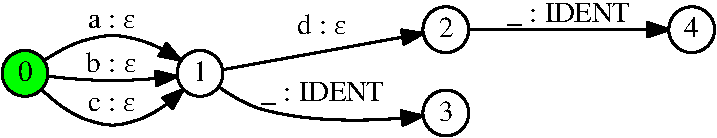
\includegraphics[width=0.45\textwidth]{pics/ident_ex}
\caption{Вершины 1 и 2 являются \textit{action}-вершинами, но из вершины 1 токен продолжает накапливаться}
\label{fig:ident_ex}
\end{figure}

Этот этап состоит из шагов, представленных ниже. В них используется структура \verb|GraphAction| (см. листинг~\ref{lst:grAct}). Эта структура предназначена для выделения токенов в конечном преобразователе $M_1$ и содержит поля для стартовой вершины, набора конечных вершин и конечного автомата. Стартовой вершиной может быть только action-вершина или начальное состояние, конечной вершиной --- action-вершина или конечное состояние. 

\fvset{frame=lines,framesep=5pt}
\begin{listing}[h]
\begin{pyglist}[language=csharp,numbers=none,numbersep=5pt]
struct GraphAction =
    int startV  
    array<int> endV
    FSA fsa  //finite state automaton
\end{pyglist}
\caption{Структура GraphAction}
\label{lst:grAct}
\end{listing}

В описании алгоритма для дуги конечного преобразователя $M_1$ используется нотация $e = (u, (a, b), v)$, где $u$ --- начальная вершина дуги, $v$ --- конечная вершина, $(a, b)$ --- метка дуги, $a \in \Sigma_1$, $y \in \Sigma'_1 \cup \{\varepsilon \}$.  Добавление дуги в конечный автомат, который содержится в структуре \verb|GraphAction|, осуществляется с помощью функции \verb|graphAction.fsa.AddEdge(e)|, которая добавляет дугу из вершины $u$ в вершину $v$, помеченную символом $a$ в соответствующий конечный автомат. В алгоритме используются очередь \textit{Q} для того, чтобы контролировать порядок обхода конечного преобразователя и структура \verb|GraphAction| \textit{grAct} для выделения конечного автомата, который содержит токен. 

\textbf{\underline{Шаг 1.}} Для конечного преобразователя $M_1$ строится набор вершин $actV$, которые являются action-вершинами. 

\textbf{\underline{Шаг 2.}} Для начального состояния конечного преобразователя $M_1$ и вершин из набора $actV$ запускается обход, который накапливает для токена конечный автомат. Порядок обхода представлен в алгоритме~\ref{algo:bfs}. Результатом обхода для всех вершин является коллекция $tokenAct$, состоящая из элементов типа \verb|GraphAction|.


\begin{algorithm}
\floatname{algorithm}{Алгоритм}
\begin{algorithmic}
\Function{bfs}{$vStart, M_1$}
\State{$grAct.startV \gets vStart$}
\State{$Q.Enqueue(vStart)$}

\While{$Q$ is not empty}
    \State{$v \gets Q.Dequeue()$}
    \If{$v$ is not visited}
        \State{\Call{visit}{v}} 
        \ForAll{$e = (v, \_, u)$ in $M_1$}
            \If{$e = (v, (\_, \varepsilon), u)$}
                \State{$c \gets$  $v$ is init state of $M_1$}
                \If{$v \neq vStart$ or $c$}
                \State{$grAct.fsa.AddEdge(e)$}
                
                \If{$u = vStart$}
                \State{$grAct.endV.Add(u)$}
                \EndIf
                \State{$Q.Enqueue(u)$}
                \EndIf
            \Else
                \If{$v = vStart$}
                \State{$grAct.fsa.AddEdge(e)$}
                    \If{$u$ is final state in $M_1$}
                        \State{$grAct.endV.Add(u)$}
                    \Else
                        \State{$Q.Enqueue(u)$}
                    \EndIf    
                \Else
                    \State{$grAct.endV.Add(v)$}
                \EndIf
            \EndIf
        \EndFor
    \EndIf
\EndWhile
\EndFunction
\caption{Порядок обхода конечного преобразователя для сохранения привязки лексических единиц к исходному коду}
\label{algo:bfs}
\end{algorithmic}
\end{algorithm}

\textbf{\underline{Шаг 3.}} Для точного определения конечного автомата, сохраняющего связь между токеном и исходным кодом, необходимо пройти конечный преобразователь $M_1$ в обратном направлении. Такая необходимость возникает в случае, если конечный преобразователь $M_1$ содержит циклы. На этом шаге также запускается обход для вершин из набора  $actV$  и начального состояния конечного преобразователя $M_2$, который является инвертированным конечным преобразователем $M_1$. Порядок обхода представлен в алгоритме~\ref{algo:bfsInv}. Результатом обхода для всех вершин является коллекция $tokenActInv$, состоящая из элементов типа \verb|GraphAction|.

\begin{algorithm}
\floatname{algorithm}{Алгоритм}
\begin{algorithmic}
\Function{bfsInv}{$vStart, M_2, M_1$}
\State{$grAct.startV \gets vStart$}
\State{$Q.Enqueue(vStart)$}

\While{$Q$ is not empty}
    \State{$v \gets Q.Dequeue()$}
    \If{$v$ is not visited}
        \State{\Call{visit}{v}} 
        \ForAll{$e = (v, \_, u)$ in $M_2$}
            \State{$grAct.fsa.AddEdge(e)$}
            \State{$c \gets $ $u$ is action-vertex or init state of $M_2$}
            \If{$c$}
                \If{$\exists e = (u, (\_, \varepsilon), \_)$ in $M_1$}
                    \State{$Q.Enqueue(u)$}
                \EndIf    
            \Else
                \State{$Q.Enqueue(u)$}
            \EndIf
        \EndFor
    \EndIf
\EndWhile
\EndFunction
\end{algorithmic}
\caption{Порядок обхода инвертированного конечного преобразователя для сохранения привязки лексических единиц к исходному коду}
\label{algo:bfsInv}
\end{algorithm}

\textbf{\underline{Шаг 4.}} Ищутся пересечения конечных автоматов, полученных на двух предыдущих шагах, при условии, что  $tokenAct.endV.current = tokenActInv.startV$. Токен определяется функцией, лежащей на дуге, исходящей из вершины $tokenAct.endV.current$, в него записывается результат пересечения. При этом в конечный автомат $A_{token}$ добавляется переход по этому токену из вершины $tokenAct.startV$ в  вершину $tokenAct.endV.current$. 

Так как символ \verb|'eof'| является вспомогательным символом для лексического анализа, то для всех вершин, из которых выходит дуга, помеченная \verb|'eof'|, добавляется переход в новое состояние по токену \verb|EOF| в конечный автомат $A_{token}$, которое теперь является конечным состоянием $A_{token}$. Над полученным конечным автоматом запускается процедура построения детерминированного конечного автомата. При этом автомат детерминирован так, чтобы на дугах из одной вершины не было двух токенов с одинаковым идентификатором и конечным автоматом.

\subsection{Пример}
Рассмотрим работу алгоритма для лексического анализа на примере. Пусть результатом аппроксимации является конечный автомат $A$, представленный на рис.~\ref{fig:calc_ex}. Для этого примера сохранение привязки для символов опускаем. 

\begin{figure}[h]
\centering
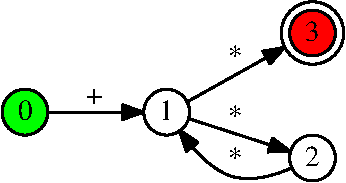
\includegraphics[width=0.3\textwidth]{pics/calc_ex}
\caption{Результат аппроксимации}
\label{fig:calc_ex}
\end{figure}

Преобразуем этот конечный автомат во входную структуру для алгоритма. Для этого сперва строится детерминированный конечный автомат $A'$ (см. рис.~\ref{fig:calc_ex_det}), затем --- конечный преобразователь $M$ (см. рис.~\ref{fig:calc_ex_fst}). 

\begin{figure}[h]
\centering
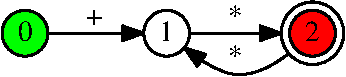
\includegraphics[width=0.3\textwidth]{pics/calc_ex_det}
\caption{Детерминированный конечный автомат $A'$}
\label{fig:calc_ex_det}
\end{figure}

\begin{figure}[h]
\centering
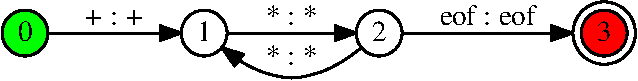
\includegraphics[width=0.4\textwidth]{pics/calc_ex_fst}
\caption{Конечный преобразователь $M$ для лексического анализа }
\label{fig:calc_ex_fst}
\end{figure}

Для обработки конечного преобразователя $M$ используется спецификация для языка арифметических выражений (см. листинг~\ref{lst:calcSpecFSA}). Результат композиции конечного преобразователя $M$ с конечным преобразователем, построенным генератором лексических анализаторов, показан на рис.~\ref{fig:calc_ex_compose}. 

\begin{figure}[h]
\centering
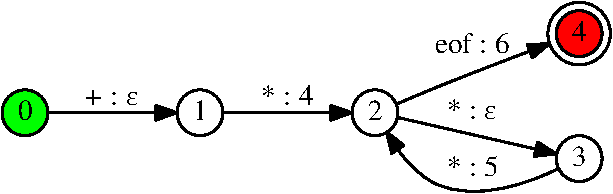
\includegraphics[width=0.4\textwidth]{pics/calc_ex_compose}
\caption{Результат композиции }
\label{fig:calc_ex_compose}
\end{figure}

На рис.~\ref{fig:calc_ex_compose} цифры соответствуют индексу в массиве действий, который представлен в листинге~\ref{lst:actFunc} (нумерация элементов в массиве начинается с 0). Индекс 4 соответствует функции, которая возвращает токен \verb|Some(PLUS)|, 5 --- токен \verb|Some(POW)|, 6 --- токен \verb|Some(MULT)|. Так как лексических ошибок получено не было, то происходит этап интерпретации полученного конечного преобразователя $M_1$, который состоит из 4 шагов. Ниже представлены результаты выполнения каждого шага.

\textbf{\underline{Шаг 1.}} В набор $actV$ добавляются action-вершины  1, 2, 3.

\textbf{\underline{Шаг 2.}} Запускается обход, представленный в алгоритме~\ref{algo:bfs}, для вершин из набора  $actV$ и вершины 0, которая является начальным состоянием конечного преобразователя $M_1$. Результатом обхода для всех вершин является коллекция $tokenAct$, которая представлена в виде таблицы~\ref{tbl:GraphAction}. 

\begin{table}[h]
  \centering
  \begin{tabular}{ | c | c | c | }
    \hline
    startV & 0 & 1 \\ \hline
    FSA
    &
    \begin{minipage}{.15\textwidth}
    \vspace{1 mm} 
      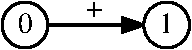
\includegraphics[width=\linewidth]{pics/0_tok}
    \end{minipage}
    &
    \begin{minipage}{.15\textwidth}
    \vspace{1 mm} 
      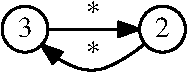
\includegraphics[width=\linewidth]{pics/24_tok}
    \end{minipage}
    \\ \hline
    endV & 1 & 2,3 \\ \hline
  \end{tabular}
  
  \vspace{2 mm}
  \begin{tabular}{ | c | c | c | }
    \hline
    startV & 2 & 3 \\ \hline
    FSA
    &
    \begin{minipage}{.15\textwidth}
    \vspace{1 mm}
      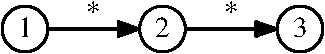
\includegraphics[width=\linewidth]{pics/20_tok}
    \end{minipage}
    & 
    \begin{minipage}{.15\textwidth}
    \vspace{1 mm}
      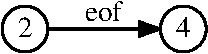
\includegraphics[width=\linewidth]{pics/35_tok}
    \end{minipage}    
    \\ \hline
    endV & 2,3 & 4
    \\ \hline
  \end{tabular}
  \caption{Коллекция $tokenAct$ для Шага 2}
  \label{tbl:GraphAction}
\end{table}

\textbf{\underline{Шаг 3.}} Запускается обход, представленный в алгоритме~\ref{algo:bfsInv}, для вершин из набора $actV$ и вершины 49, которая является начальным состоянием конечного преобразователя $M_2$. Результатом обхода для всех вершин является коллекция $tokenActInv$, которая представлена в виде таблицы~\ref{tbl:GraphActionInv}. 

\begin{table}[t]
  \centering
  \begin{tabular}{| c | c | c | }
    \hline
    startV & 1 & 3  \\ \hline
    FSA 
    &
    \begin{minipage}{.15\textwidth}
    \vspace{1 mm} 
      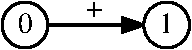
\includegraphics[width=\linewidth]{pics/0_tok}
    \end{minipage}
    &
    \begin{minipage}{.15\textwidth}
    \vspace{1 mm} 
      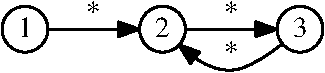
\includegraphics[width=\linewidth]{pics/24_inv}
    \end{minipage}
    \\ \hline
   \end{tabular}
  
  \vspace{2 mm}
  \begin{tabular}{ | c | c | c | }
  \hline
    startV & 2 & 4 \\ \hline
    FSA
    &
    \begin{minipage}{.15\textwidth}
    \vspace{1 mm}
      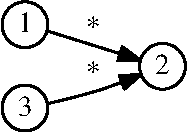
\includegraphics[width=0.7\linewidth]{pics/35_inv}
    \end{minipage}
    & 
    \begin{minipage}{.15\textwidth}
    \vspace{1 mm} 
      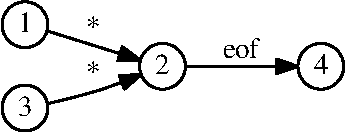
\includegraphics[width=\linewidth]{pics/49_inv}
    \end{minipage}    
    \\ \hline
  \end{tabular}
  \caption{Коллекция $tokenActInv$ для Шага 3}
  \label{tbl:GraphActionInv}
\end{table}

\textbf{\underline{Шаг 4.}} Выполняются операции пересечения конечных автоматов, результаты которых представлен в таблице~\ref{tbl:GraphActionInters}.


\begin{table}[h]
  \centering
  \begin{tabular}{ | c | c |}
    \hline 
    \begin{minipage}{.2\textwidth}
    \vspace{1 mm}
      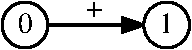
\includegraphics[width=\linewidth]{pics/0_tok}
    \end{minipage}
    &
    \begin{minipage}{.2\textwidth}
    \vspace{1 mm}
      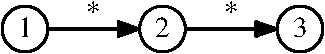
\includegraphics[width=\linewidth]{pics/20_tok}
    \end{minipage}
    \\ \hline
    
    \begin{minipage}{.2\textwidth}
    \vspace{1 mm}
      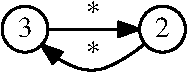
\includegraphics[width=\linewidth]{pics/24_tok}
    \end{minipage}
    &
    \begin{minipage}{.2\textwidth}
    \vspace{1 mm} 
      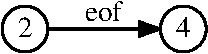
\includegraphics[width=\linewidth]{pics/35_tok}
    \end{minipage}
    \\ \hline
    
    \begin{minipage}{.2\textwidth}
    \vspace{1 mm}
      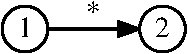
\includegraphics[width=\linewidth]{pics/20_int}   
    \end{minipage}
    & 
    \begin{minipage}{.2\textwidth}
    \vspace{1 mm}
      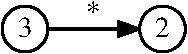
\includegraphics[width=\linewidth]{pics/24_int}
    \end{minipage}
    \\ \hline
  \end{tabular}
  \caption{Результат пересечения конечных автоматов из таблиц~\ref{tbl:GraphAction} и ~\ref{tbl:GraphActionInv}}
  \label{tbl:GraphActionInters}
\end{table}

Результатом лексического анализа будет конечный автомат, представленный на рис.~\ref{fig:calc_ex_res}. Каждая дуга графа содержит токен, который хранит в себе конечный автомат. Например, дуга от вершины 1 к вершине 3 содержит токен \verb|POW|, у которого хранится конечный автомат с переходами от состояния 1 к состоянию 2 по символу '*', от 2 к 3 --- по символу '*', полученный в результате пересечения конечных автоматов. 

\begin{figure}[H]
\centering
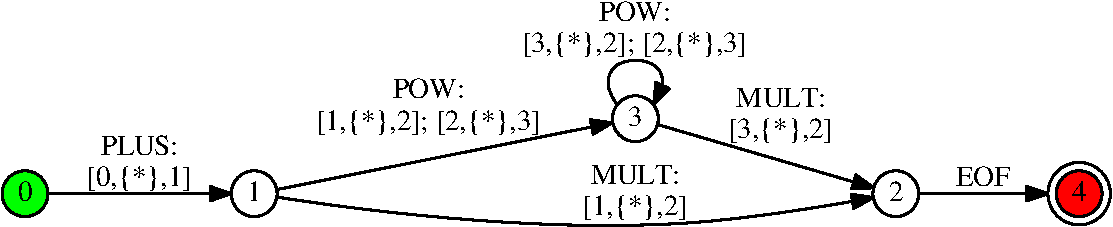
\includegraphics[width=0.5\textwidth]{pics/calc_ex_res}
\caption{Результат лексического анализа }
\label{fig:calc_ex_res}
\end{figure}

\section{Архитектура модуля для лексического анализа}
Архитектура инструмента, реализующая рассмотренный механизм, представлена на рис.~\ref{fig:ComponentDiagram_rus}. 

\begin{figure}[H]
\centering
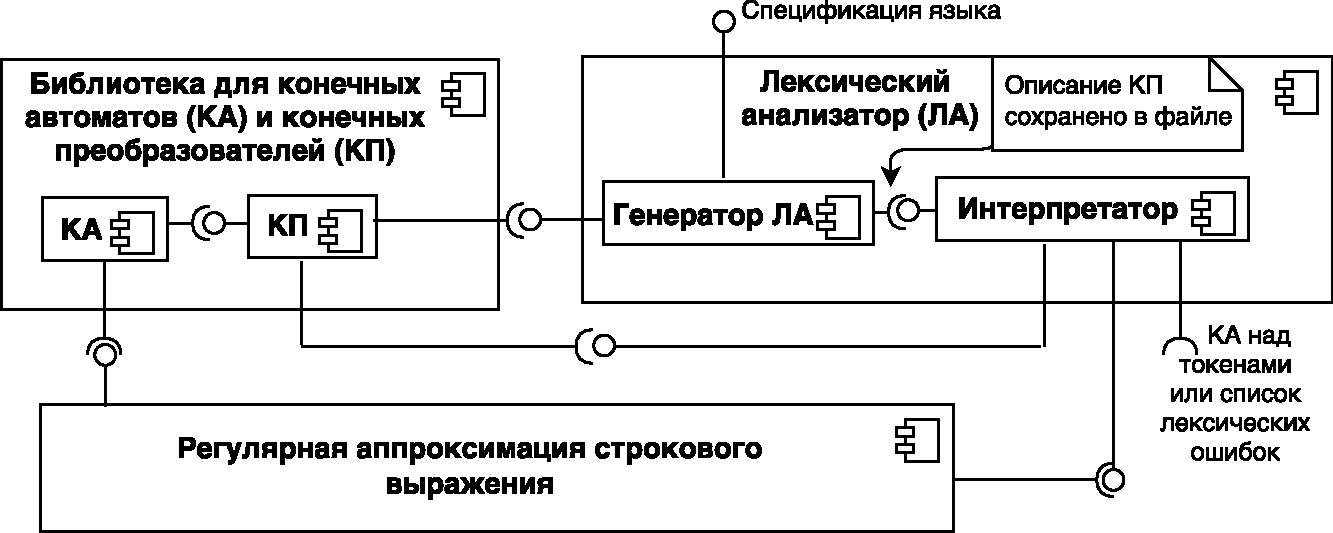
\includegraphics[width=0.48\textwidth]{pics/architecture_module}
\caption{Архитектура модуля для лексического анализа}
\label{fig:ComponentDiagram_rus}
\end{figure}

Компонента \textbf{Лексический анализатор} состоит из \textbf{Генератора лексических анализаторов} и \textbf{Интерпретатора}. Генератор лексических анализаторов строит конечный преобразователь, описание которого взято из \textbf{Библиотеки для конечных автоматов и конечных преобразователей}, и сохраняет результат в отдельный файл. Такой подход позволяет многократно использовать данный конечный преобразователь для обработки кода, написанного на одном языке. \textbf{Интерпретатор} принимает на вход два конечных преобразователя, один из которых из которых получен в результате построения аппроксимации (за это отвечает компонент \textbf{Регулярная аппроксимация строкового выражения}), а второй построен генератором лексических анализаторов. Результатом работы \textbf{Интерпретатора} является либо конечный автомат над алфавитом токенов эталонной грамматики языка, либо список обнаруженных лексических ошибок. 

\textbf{Библиотека для конечных автоматов и конечных преобразователей} предоставляет ряд операций, которые необходимы для построения аппроксимации и проведения лексического анализа. Для конечных автоматов используются операции: конкатенация, replace, дополнение, пересечение,  а для конечных преобразователей --- композиция. 

\section{Апробация}

В данном разделе описан механизм использования реализованного инструмента, а также рассмотрены примеры, демонстрирующие разработанную функциональность.

Для осуществления лексического разбора необходимо выполнить следующие шаги.

\textbf{\underline{Шаг 1.}} Запустить генератор, указав путь к файлу с расширением .fsl, в котором написана спецификация. В результате создается файл с расширением .fs, содержащий конечный преобразователь и вспомогательные функции.

\textbf{\underline{Шаг 2.}} Необходимо в отдельном файле с расширением .fs указать описание типов токенов, которые автоматически строятся по грамматике эталонного языка. Полученные файлы подключить в модуль, предназначенный для получения результата лексического разбора. 

\textbf{\underline{Шаг 3.}} Получить конечный автомат, аппроксимирующий множество значений строкового выражения и удовлетворяющий описанию используемой библиотеки для конечных автоматов и конечных преобразователей. Преобразовать этот конечный автомат в конечный преобразователь (см. Алгоритм лексического анализа).

\textbf{\underline{Шаг 4.}}  Вызвать функцию \verb|tokenize| из сгенерированного файла. Результатом этой функции будет либо конечный автомат над алфавитом токенов эталонной грамматики языка, либо список лексических ошибок. 

Рассмотрим примеры, которые показывают преимущества реализованного решения, а именно, возможность сохранения конечного автомата внутри структуры токена и обработки циклов во входном конечном автомате. 

\textbf{\underline{Пример 1.}}
Рассмотрим следующий пример кода:
\fvset{frame=lines,framesep=5pt}
\begin{listing}[H]
\begin{pyglist}[language=csharp,numbers=none,numbersep=5pt]
private void Go(int number){
   String query = 
        "SELECT nameX FROM tableY WHERE x < ";
   while(query.Length < number){
      query += "+ 1 ";
   }
   Program.ExecuteImmediate(query);
}
\end{pyglist}
\caption{Пример формирования выражения в цикле}
\label{lst:exampleWhile}
\end{listing}

Результатом аппроксимации выражения \verb|query| является конечный автомат, представленный на рис.~\ref{fig:while_appr}. Результат лексического анализа представлен на рис.~\ref{fig:while_lex}. В результирующем конечном автомате учитываются две ситуации: цикл не выполняется (путь $0 \to \ldots \to 7 \to 9$) и выполняется (путь $0 \to \ldots \to 7 \to 8 \to 10 \to 8 \to \ldots \to 10 \to 9$), что позволяет уточнить проводимый анализ в целом. 

\begin{figure}[h]
\centering
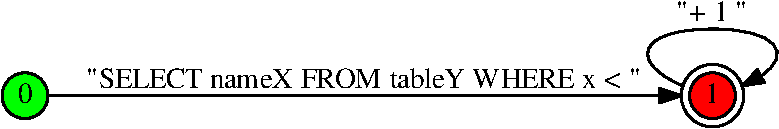
\includegraphics[width=0.45\textwidth]{pics/while_appr}
\caption{Результат аппроксимации}
\label{fig:while_appr}
\end{figure}


\begin{figure}[h]
\centering
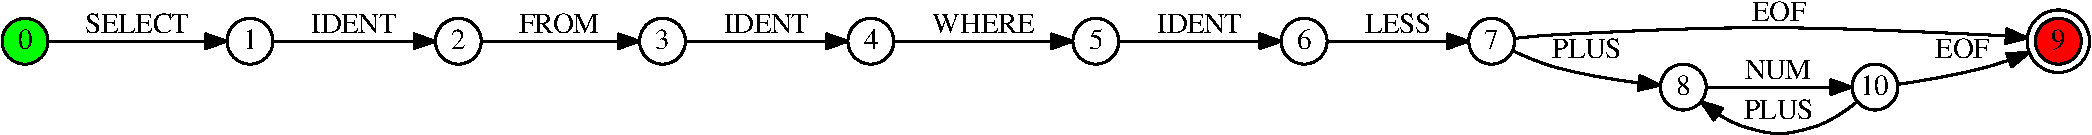
\includegraphics[width=0.5\textwidth]{pics/WhileEx}
\caption{Результат лексического анализа}
\label{fig:while_lex}
\end{figure}

\textbf{\underline{Пример 2.}}
Рассмотрим следующий пример кода, в котором конечный автомат токена содержит цикл:
\fvset{frame=lines,framesep=5pt}
\begin{listing}[H]
\begin{pyglist}[language=csharp,numbers=none,numbersep=5pt]
String query = "SELECT name";
for(int i = 0; i < 10; i++){
   query  += "X";
}
query += " FROM tableY";
Program.ExecuteImmediate(query);
\end{pyglist}
\caption{Пример кода, в котором конечный автомат токена содержит цикл}
\label{lst:exampleFor}
\end{listing}

Результатом лексического анализа будет конечный автомат, представленный на рис.~\ref{fig:token_ex}. Конечный автомат первого токена \verb|IDENT|, содержащий цикл, представлен на рис.~\ref{fig:token_lex}. На этом же рисунке показана сохраненная привязка символов к исходному коду. Таким образом, если цикл содержится только в конечном автомате токена, то в результирующем конечном автомате циклы отсутствуют, что позволяет упростить структуру входных данных для дальнейшего анализа.

\begin{figure}[h]
\centering
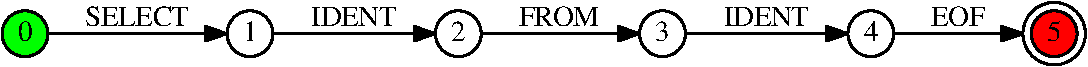
\includegraphics[width=0.5\textwidth]{pics/TokenEx}
\caption{Результат лексического анализа}
\label{fig:token_ex}
\end{figure}

\begin{figure}[h]
\centering
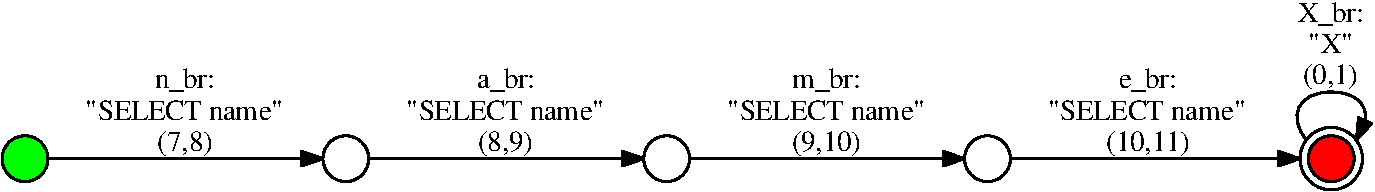
\includegraphics[width=0.5\textwidth]{pics/token}
\caption{Конечный автомат первого токена IDENT, содержащий цикл}
\label{fig:token_lex}
\end{figure}

На практике основным сценарием для динамически формируемого выражения является следующая ситуация, где строки x1, x2, \ldots, xn возвращают одинаковый идентификатор токена:

\begin{figure}[h]
\centering
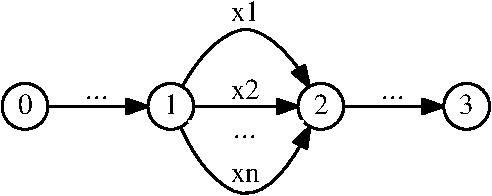
\includegraphics[width=0.4\textwidth]{pics/n_ex}
\caption{Конечный автомат}
\label{fig:fsa_n}
\end{figure}

Разработанный механизм лексического анализа вернет один токен при переходе от состояния 1 к  состоянию 2, что значительно упрощает входные данные для синтаксического разбора.

\section{Заключение}
% * <Семён Григорьев> 13:49:55 12 Aug 2015 UTC+0300:
% Ничего не мказано про генератор.
% ^ <Марина Полубелова> 17:14:02 12 Aug 2015 UTC+0300:
% А что про него сказать? Он все-таки упомянут: описан генератор ЛА в данной работе)
% ^ <Семён Григорьев> 17:20:38 12 Aug 2015 UTC+0300:
% Надо как-то более явно сказать, что генератор -- штука таки полезная и он тоже результат.

В данной работе описан алгоритм лексического анализа и основанный на нем генератор лексических анализаторов для динамически формируемого кода. Данный алгоритм был реализован в проекте YaccConstructor на языке программирования F\#. Разработанный алгоритм позволяет при проведении лексического анализа для токена сохранять конечный автомат, что значительно упрощает входные данные для синтаксического разбора. Также алгоритм позволяет хранить привязку лексических единиц к исходному коду, которая необходима для позиционирования места ошибок или навигации по коду. 

Разработанный генератор лексических анализаторов позволяет получать по спецификации языка соответствующий анализатор, использующий описанный алгоритм. Таким образом, был разработан автоматизированный подход создания лексических анализаторов для динамически формируемого кода.

В дальнейшем планируется снять ограничения на формат написания спецификации, по которому генератор лексических анализаторов строит соответствующий анализатор, а также оптимизировать полученный инструмент  за счет подбора структур данных и алгоритмов для работы с конечными автоматами~\cite{AlgoFSA}.

\nocite{*}
\def\BibTeX{BibTeX}
\bibliographystyle{IEEEtran}

\bibliography{IEEEabrv,./IEEEexample}
\end{document}
